\clearpage
\section{Specyfikacja programowo-sprzętowa}
\label{sec:spec_prog}

\subsection{Sprzęt}
\quad W przypadku tak stricte programowego projektu, jak opisywany w niniejszym raporcie ciężko jest wyróżnić jakąś szczególną specyfikację potrzebnego sprzętu. Do realizacji wykorzystywaliśmy tylko komputer klasy PC z oprogramowaniem opisanym w podrozdziale \ref{sub:plat_prog}.

To, o czym jednak należy tutaj wspomnieć, to używane zwykle w synchrotronach zestawy silników krokowych, które mają specyficzne możliwości konfiguracyjne oraz mogą być prosto zintegrowane z rozproszonym systemem sterowania zarządzanym przy pomocy narzędzi Tango. Najczęściej stosowanym rozwiązaniem jest platforma programowo - sprzętowa IcePAP \cite{web:icepap, proc:icepap}.

\subsection{Platformy programowe}
\label{sub:plat_prog}

\begin{enumerate}
	\item \textbf{Tango}
	
	\hspace{2em}System sterowania TANGO jest darmowym zestawem narzędzi do sterowania dowolnego rodzaju sprzętem lub oprogramowaniem oraz do budowy systemów SCADA (ang. Supervisory Control And Data Acquisition). Jest to oprogramowanie typu open-source wykorzystywane do sterowania synchrotronami, laserami oraz innymi eksperymentami fizycznymi. TANGO jest aktywnie rozwijane przez TANGO Consortium.
	
	\hspace{2em}TANGO jest rozproszonym systemem sterowania. Oznacza to, że może działać zarówno na jednej maszynie, jak i na wielu. Wykorzystuje dwa protokoły sieciowe - COBRA oraz Zeromq. Podstawowym modelem komunikacji jest model klient-serwer. Komunikacja pomiędzy klientem i serwerem może być synchroniczna, asynchroniczna (COBRA) oraz sterowana zdarzeniem (Zeromq) \cite{TangoWiki}. Schemat ideowy całości oprogramowania dostępnego w ramach projektu Tango jest pokazany na rys. \ref{fig:tango-outline}. Jest na nim zaprezentowany podział na pakiety do budowania aplikacji klienckich, programy służące do zarządzania, archiwizację, centralną bazę danych (pod sekcją TANGO HOST) oraz mnogość urządzeń skomunikowanych z resztą systemu przez dedykowane interfejsy programowej magistrali - serwery urządzeń (ang. Device Servers).
	
	\begin{figure}[hpt]
		\centering
		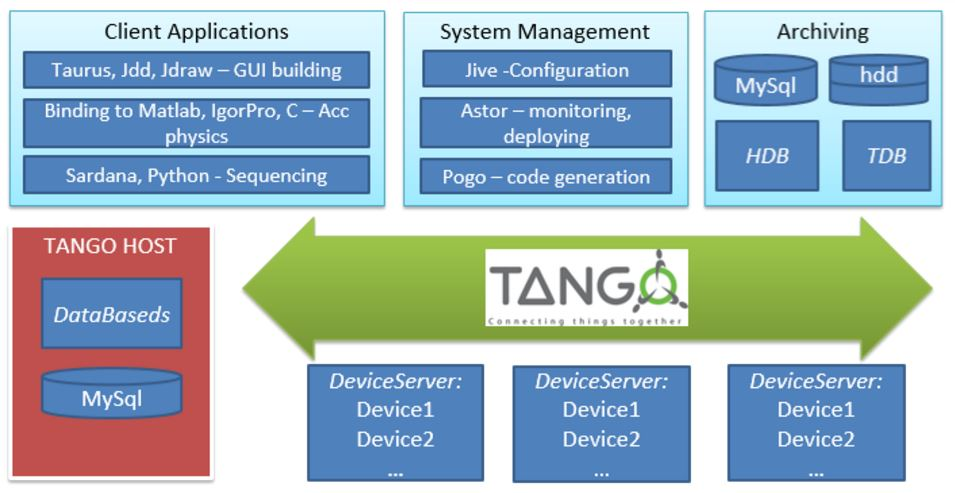
\includegraphics[width=1\linewidth]{Grafika/tango_outline}
		\caption{Schemat ideowy różnych komponentów systemu sterowania Tango. Wykonanie schematu: Piotr Goryl, NCPS Solaris.}
		\label{fig:tango-outline}
	\end{figure}
	
	\hspace{2em}System TANGO jest opakowaniem (ang. wrapper) dla protokołu COBRA zapewniającym przyjazne dla użytkownika API. Dzięki takiemu podejsciu wiele detali związanych z nawiązywaniem i utrzymywaniem połączenia pomiędzy urządzeniami jest niewidoczna dla użytkownia, co pozwala na szybsze i łatwiejsze rozbudowywanie systemu sterowania.
	
	\hspace{2em}TANGO wykorzystuje MySQL jako bazę danych do trzymania informacji. Informacjami takimi mogą byc np. nazwy urządzeń, adresy sieciowe, listy urządzeń itp. MySQL jest relacyjną bazą danych implementującą podzbiór SQLa. System TANGO jest wspierany przez 4 platformy: Linux, Windows NT, Solaris oraz HP-UX.
	
	\begin{enumerate}
		\item \textbf{Taurus}
		
		\hspace{2em}Taurus jest platformą programistyczną dla Pythona służącą do sterowania oraz akwizycji danych w zastosowaniach naukowych oraz przemysłowych. Pozwala na szybkie i proste tworzenie interfejsów użytkownika. Jest to częśc pakietu programistycznego Sardana. Taurus posiada bogatą bibliotekę dzięki czemu stworzone GUI (ang. Graphical User Interface)  może zawierać wiele różnych komponentów takich jak wykresy, tabele, przyciski itp. Celem biblioteki Taurus jest zapewnienie przyjaznego API dla użytkownika oraz przyspieszenie procesu rozwijania aplikacji bazowanych na TANGO. Jeden z paneli w czasie konfigurowania nowego GUI jest przedstawiony na rys. \ref{fig:taurusgui}.
		
		\begin{figure}[pth]
			\centering
			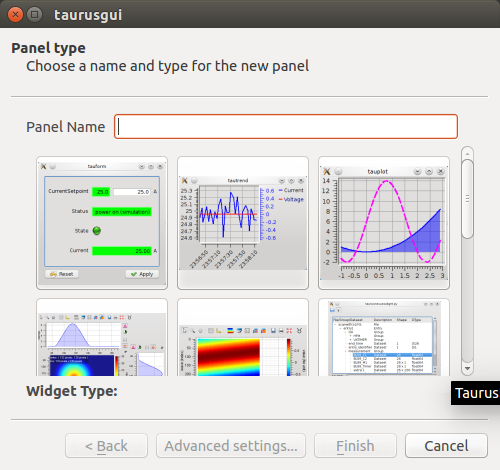
\includegraphics[width=0.6\linewidth]{Grafika/taurusgui}
			\caption{Zrzut ekranu pokazujący tworzenie nowego GUI za pomocą TaurusGUI.}
			\label{fig:taurusgui}
		\end{figure}
				
		
		\item \textbf{Sardana}
		
		\hspace{2em}Sardana to pakiet oprogramowania do nadzoru, kontroli i akwizycja danych w zastosowaniach naukowych. Jej celem jest zredukowanie kosztów oraz czasu potrzebnych do projektowania, rozwijania oraz utrzymywania systemów SCADA. Rozwój Sardany zapoczątkowany został przy synchrotronie ALBA, a dzisiaj jest wspierany przez wiekszą społeczność,  w skład której wchodzą liczne laboratoria oraz inne jednostki (ALBA, DESY, MaxIV, Solaris, ESRF).
		Sardana jest bazowana na systemie TANGO i wykorzystuje bibliotekę Taurus umożliwiającą programowanie i konfigurację interfejsu użytkownika \cite{Sardana}.
		
		\item \textbf{Narzędzia pakietu TANGO}
		
		\hspace{2em}Najważniejszymi narzędziami pakietu TANGO są Jive oraz Astor. Pierwsze z nich jest wykorzystywane do zarządzania urządzeniami - ich właściwościami, okresem odpytywania, nazwami, wyświetlanymi parametrami, itp. Zostało zaprezentowane na rys. \ref{fig:jive}. Umożliwia również uruchomienie panelu wszystkich atrybutów i komend pojedynczego urządzenia - aplikacji ATKPanel (jest ona pokazana na rys. \ref{fig:atk}).
		
		\begin{figure}[pth]
			\centering
			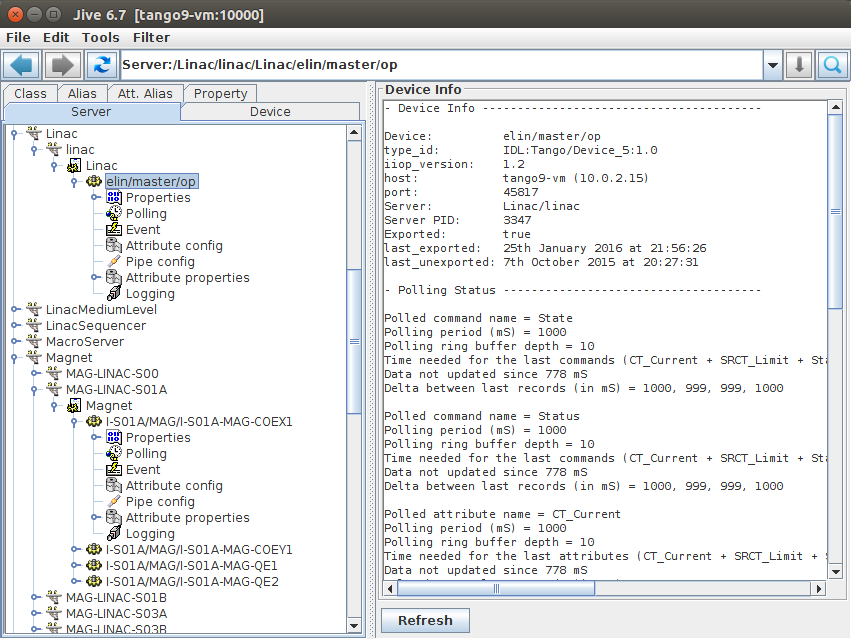
\includegraphics[width=1\linewidth]{Grafika/jive}
			\caption{Zrzut ekranu pokazujący aplikację Jive.}
			\label{fig:jive}
		\end{figure}
		
		\begin{figure}[pth]
			\centering
			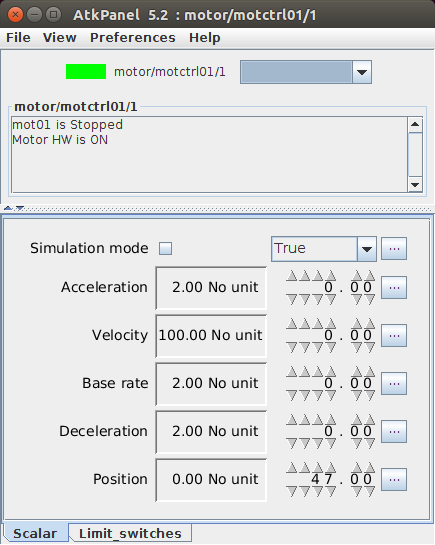
\includegraphics[width=0.5\linewidth]{Grafika/atk}
			\caption{Zrzut ekranu pokazujący aplikację ATKPanel.}
			\label{fig:atk}
		\end{figure}
		
		\hspace{2em}Drugie - Astor - służy do zarządzania serwerami urządzeń oraz maszynami, na których owe serwery są uruchamiane. Możemy je logicznie grupować, włączać, resetować, testować czy sprawdzać logi. Wygląd panelu dla pojedynczej maszyny z serwerami jest pokazany na rys. \ref{fig:astor}.
		
		\begin{figure}[pth]
			\centering
			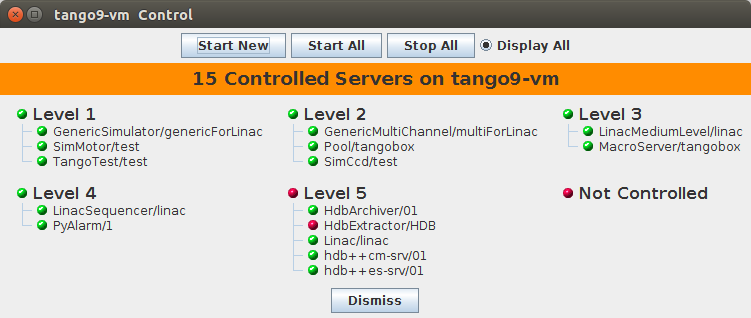
\includegraphics[width=1\linewidth]{Grafika/astor_panel}
			\caption{Zrzut ekranu pokazujący panel aplikacji Astor.}
			\label{fig:astor}
		\end{figure}
		
		\item \textbf{TangoBox9} (maszyna wirtualna)
		
		W związku z polityką udostępniania oprogramowania na otwartych licencjach, konsorcjum Tango wypuściło gotową wirtualną maszynę, która zawiera wszystkie narzędzia pakietu Tango zainstalowane na systemie Ubuntu 14.04 64-bit. Są tam uwzględnione również wszystkie poboczne projekty, które ułatwiają korzystanie z systemu i dostarczają dodatkowych opcji potrzebnych systemowi sterowania, np. archiwizacji, logowania czy tworzenia interfejsów użytkownika. W tym systemie dostarczono w pełni funkcjonalne symulacyjne środowisko systemu sterowania synchrotronem z uwzględnieniem jednej linii badawczej. Obecne są tam również podstawowe aplikacje będące częścią bazowej paczki Tango, takie jak: Astor, Pogo (generator kodu serwerów), Jive czy AtkMoni (umożliwiają konfigurację i testowanie samych urządzeń).
		
	\end{enumerate}
	\item \textbf{Python}
	
	\hspace{2em}Python to wysokopoziomowy język programowania ogólnego przeznaczenia. Posiada rozbudowane pakiety bibliotek standardowych. Ideą przewodnią Pythona jest czytelność i klarowność kodu źródłowego. Jego składnia cechuje się przejrzystością i zwięzłością. W Pythonie możliwe jest programowanie obiektowe, programowanie strukturalne i programowanie funkcyjne. Typy sprawdzane są dynamicznie, a do zarządzania pamięcią stosuje się garbage collection. Python rozprowadzany jest na otwartej licencji umożliwiając także zastosowanie do zamkniętych komercyjnych projektów \cite{Python}.
	
	\begin{enumerate}
		\item \textbf{PyCharm}
		
		\hspace{2em}PyCharm to zintegrowane środowisko programistyczne (IDE) dla języku programowania Python firmy JetBrains. Zapewnia m.in.: edycję i analizę kodu źródłowego, graficzny debugger, uruchamianie testów jednostkowych, integrację z systemem kontroli wersji. Wspiera także programowanie i tworzenie aplikacji internetowych w Django.
		
		\hspace{2em}Jest oprogramowaniem wieloplatformowym pracującym na platformach systemowych: Microsoft Windows, Linux oraz OS X. Wydawany jest w wersji Professional Edition, które jest oprogramowaniem zamkniętym oraz w wersji darmowej Community Edition, które pozbawione jest jednak niektórych funkcjonalności w porównaniu z wersją komercyjną \cite{PyCharm}.
		
	\end{enumerate}
	\item \textbf{QtDesigner}
	
	\hspace{2em}Jest to narzędzie slużące do projektowania graficznego interfejsu użytkownika (GUI), zawarte w wieloplatformowym środowisku programistycznym Qt Creator. Jego wygląd jest pokazany na rys. \ref{fig:taurusdesigner}. Jak widać, można do niego zaimportować zestaw widżetów z biblioteki Taurus - wtedy komponowanie graficzne aplikacji klienckich w systemie Tango staje się bardzo proste. Podstawowe funkcje tego pakietu to:
	\begin{enumerate}
		\item tworzenie różnych typów GUI (głównych okien, pojedynczych paneli, okienek dialogowych, itp.),
		\item dodawanie różnych rodzajów widżetów,
		\item układanie graficzne wybranych elementów,
		\item edytowanie ich właściwości,
		\item zapis w formacie .ui, umożliwiającym późniejsze importowanie do aplikacji w języku C++ lub Python bądź bezpośrednią konwersję na kod w tym drugim języku.
	\end{enumerate}
\end{enumerate}

\begin{figure}[ht]
	\begin{adjustbox}{addcode={
				\begin{minipage}{\width}}
				{\caption{Zrzut ekranu pokazujący aplikację QtDesigner.}\label{fig:taurusdesigner}
				\end{minipage}},rotate=90,center}
			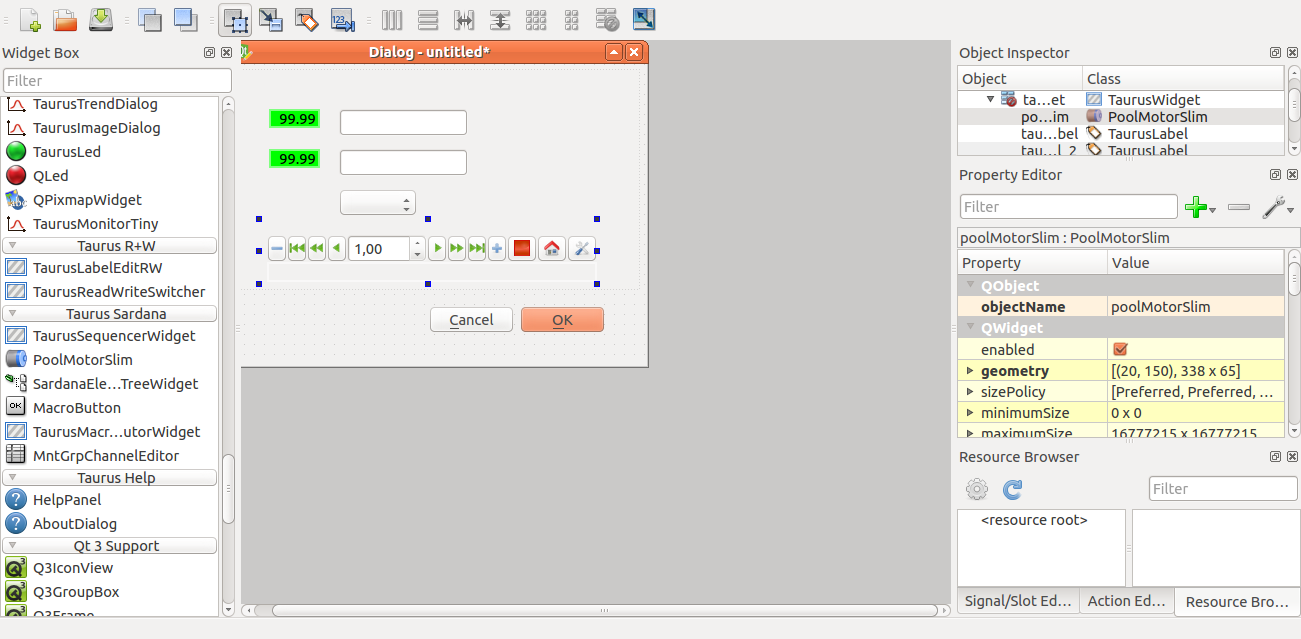
\includegraphics[scale=.45]{Grafika/taurus_designer}
		\end{adjustbox}
	\end{figure}